\documentclass{standalone}
\usepackage{tikz}
\usetikzlibrary{patterns, positioning}


\begin{document}
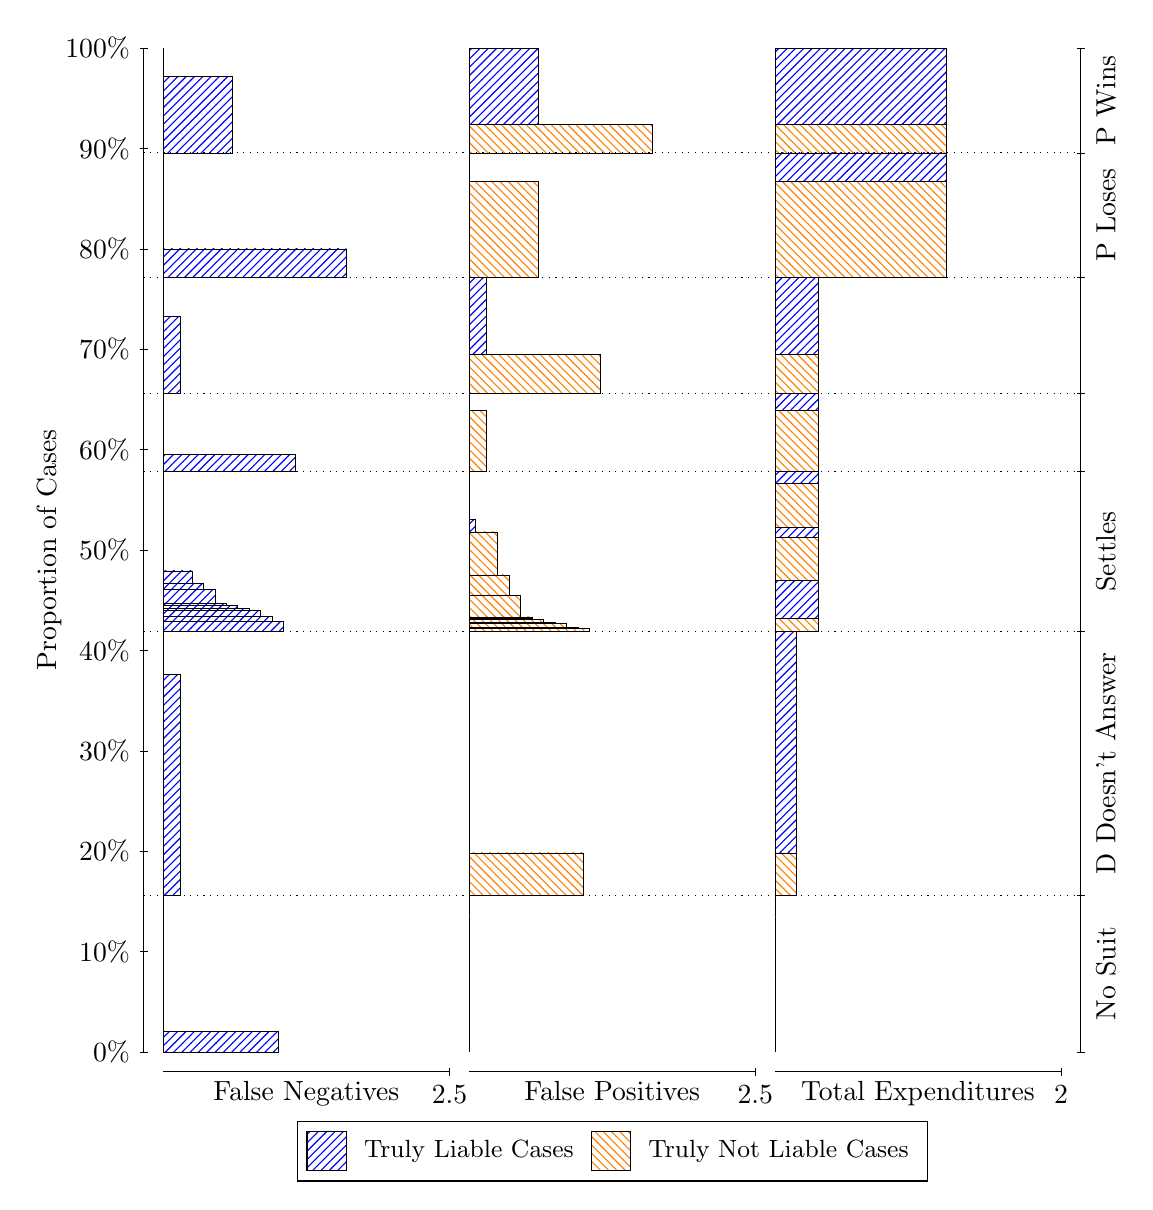
\begin{tikzpicture}
\draw[black, very thin] (1.5,1.75) -- (1.5,14.5);
\node[rotate=90, text=black, anchor=center] at (0.3, 8.125) {Proportion of Cases};
\draw[black, very thin] (1.45,1.75) -- (1.55,1.75);
\node[text=black, anchor=east] at (1.45, 1.75) {0\%};
\draw[black, very thin] (1.45,3.025) -- (1.55,3.025);
\node[text=black, anchor=east] at (1.45, 3.025) {10\%};
\draw[black, very thin] (1.45,4.3) -- (1.55,4.3);
\node[text=black, anchor=east] at (1.45, 4.3) {20\%};
\draw[black, very thin] (1.45,5.575) -- (1.55,5.575);
\node[text=black, anchor=east] at (1.45, 5.575) {30\%};
\draw[black, very thin] (1.45,6.85) -- (1.55,6.85);
\node[text=black, anchor=east] at (1.45, 6.85) {40\%};
\draw[black, very thin] (1.45,8.125) -- (1.55,8.125);
\node[text=black, anchor=east] at (1.45, 8.125) {50\%};
\draw[black, very thin] (1.45,9.4) -- (1.55,9.4);
\node[text=black, anchor=east] at (1.45, 9.4) {60\%};
\draw[black, very thin] (1.45,10.675) -- (1.55,10.675);
\node[text=black, anchor=east] at (1.45, 10.675) {70\%};
\draw[black, very thin] (1.45,11.95) -- (1.55,11.95);
\node[text=black, anchor=east] at (1.45, 11.95) {80\%};
\draw[black, very thin] (1.45,13.225) -- (1.55,13.225);
\node[text=black, anchor=east] at (1.45, 13.225) {90\%};
\draw[black, very thin] (1.45,14.5) -- (1.55,14.5);
\node[text=black, anchor=east] at (1.45, 14.5) {100\%};

\draw[black, very thin] (13.4,1.75) -- (13.4,14.5);
\draw[black, very thin] (13.35,1.75) -- (13.45,1.75);
\node[anchor=west] at (13.35, 1.75) {};
\draw[black, very thin] (13.35,3.7378) -- (13.45,3.7378);
\node[anchor=west] at (13.35, 3.7378) {};
\draw[black, very thin] (13.35,7.0909) -- (13.45,7.0909);
\node[anchor=west] at (13.35, 7.0909) {};
\draw[black, very thin] (13.35,9.1246) -- (13.45,9.1246);
\node[anchor=west] at (13.35, 9.1246) {};
\draw[black, very thin] (13.35,10.115) -- (13.45,10.115);
\node[anchor=west] at (13.35, 10.115) {};
\draw[black, very thin] (13.35,11.585) -- (13.45,11.585);
\node[anchor=west] at (13.35, 11.585) {};
\draw[black, very thin] (13.35,13.168) -- (13.45,13.168);
\node[anchor=west] at (13.35, 13.168) {};
\draw[black, very thin] (13.35,14.5) -- (13.45,14.5);
\node[anchor=west] at (13.35, 14.5) {};

\draw[black, very thin, pattern color=blue, pattern=north east lines] (1.75,1.75) rectangle (3.2033,2.0159);
\draw[black, very thin, pattern color=orange, pattern=north west lines] (1.75,2.0159) rectangle (1.75,3.7378);
\draw[black, very thin, pattern color=blue, pattern=north east lines] (1.75,3.7378) rectangle (1.968,6.549);
\draw[black, very thin, pattern color=orange, pattern=north west lines] (1.75,6.549) rectangle (1.75,7.0909);
\draw[black, very thin, pattern color=blue, pattern=north east lines] (1.75,7.0909) rectangle (3.276,7.219);
\draw[black, very thin, pattern color=blue, pattern=north east lines] (1.75,7.219) rectangle (3.1307,7.2823);
\draw[black, very thin, pattern color=blue, pattern=north east lines] (1.75,7.2823) rectangle (2.9853,7.3581);
\draw[black, very thin, pattern color=blue, pattern=north east lines] (1.75,7.3581) rectangle (2.84,7.3874);
\draw[black, very thin, pattern color=blue, pattern=north east lines] (1.75,7.3874) rectangle (2.6947,7.4242);
\draw[black, very thin, pattern color=blue, pattern=north east lines] (1.75,7.4242) rectangle (2.5493,7.4467);
\draw[black, very thin, pattern color=blue, pattern=north east lines] (1.75,7.4467) rectangle (2.404,7.6241);
\draw[black, very thin, pattern color=blue, pattern=north east lines] (1.75,7.6241) rectangle (2.2587,7.7058);
\draw[black, very thin, pattern color=blue, pattern=north east lines] (1.75,7.7058) rectangle (2.1133,7.8596);
\draw[black, very thin, pattern color=orange, pattern=north west lines] (1.75,7.8596) rectangle (1.75,9.1246);
\draw[black, very thin, pattern color=blue, pattern=north east lines] (1.75,9.1246) rectangle (3.4213,9.3414);
\draw[black, very thin, pattern color=orange, pattern=north west lines] (1.75,9.3414) rectangle (1.75,10.115);
\draw[black, very thin, pattern color=blue, pattern=north east lines] (1.75,10.115) rectangle (1.968,11.094);
\draw[black, very thin, pattern color=orange, pattern=north west lines] (1.75,11.094) rectangle (1.75,11.585);
\draw[black, very thin, pattern color=blue, pattern=north east lines] (1.75,11.585) rectangle (4.0753,11.949);
\draw[black, very thin, pattern color=orange, pattern=north west lines] (1.75,11.949) rectangle (1.75,13.168);
\draw[black, very thin, pattern color=blue, pattern=north east lines] (1.75,13.168) rectangle (2.622,14.137);
\draw[black, very thin, pattern color=orange, pattern=north west lines] (1.75,14.137) rectangle (1.75,14.5);
\draw[black, very thin, pattern color=orange, pattern=north west lines] (5.6333,1.75) rectangle (5.6333,3.4719);
\draw[black, very thin, pattern color=blue, pattern=north east lines] (5.6333,3.4719) rectangle (5.6333,3.7378);
\draw[black, very thin, pattern color=orange, pattern=north west lines] (5.6333,3.7378) rectangle (7.0867,4.2797);
\draw[black, very thin, pattern color=blue, pattern=north east lines] (5.6333,4.2797) rectangle (5.6333,7.0909);
\draw[black, very thin, pattern color=orange, pattern=north west lines] (5.6333,7.0909) rectangle (7.1593,7.1256);
\draw[black, very thin, pattern color=orange, pattern=north west lines] (5.6333,7.1256) rectangle (7.014,7.1451);
\draw[black, very thin, pattern color=orange, pattern=north west lines] (5.6333,7.1451) rectangle (6.8687,7.1886);
\draw[black, very thin, pattern color=orange, pattern=north west lines] (5.6333,7.1886) rectangle (6.7233,7.21);
\draw[black, very thin, pattern color=orange, pattern=north west lines] (5.6333,7.21) rectangle (6.578,7.2461);
\draw[black, very thin, pattern color=orange, pattern=north west lines] (5.6333,7.2461) rectangle (6.4327,7.2568);
\draw[black, very thin, pattern color=orange, pattern=north west lines] (5.6333,7.2568) rectangle (6.4327,7.2763);
\draw[black, very thin, pattern color=orange, pattern=north west lines] (5.6333,7.2763) rectangle (6.2873,7.5505);
\draw[black, very thin, pattern color=orange, pattern=north west lines] (5.6333,7.5505) rectangle (6.142,7.8086);
\draw[black, very thin, pattern color=orange, pattern=north west lines] (5.6333,7.8086) rectangle (5.9967,8.3559);
\draw[black, very thin, pattern color=blue, pattern=north east lines] (5.6333,8.3559) rectangle (5.706,8.5096);
\draw[black, very thin, pattern color=blue, pattern=north east lines] (5.6333,8.5096) rectangle (5.6333,9.1246);
\draw[black, very thin, pattern color=orange, pattern=north west lines] (5.6333,9.1246) rectangle (5.8513,9.8986);
\draw[black, very thin, pattern color=blue, pattern=north east lines] (5.6333,9.8986) rectangle (5.6333,10.115);
\draw[black, very thin, pattern color=orange, pattern=north west lines] (5.6333,10.115) rectangle (7.3047,10.606);
\draw[black, very thin, pattern color=blue, pattern=north east lines] (5.6333,10.606) rectangle (5.8513,11.585);
\draw[black, very thin, pattern color=orange, pattern=north west lines] (5.6333,11.585) rectangle (6.5053,12.803);
\draw[black, very thin, pattern color=blue, pattern=north east lines] (5.6333,12.803) rectangle (5.6333,13.168);
\draw[black, very thin, pattern color=orange, pattern=north west lines] (5.6333,13.168) rectangle (7.9587,13.531);
\draw[black, very thin, pattern color=blue, pattern=north east lines] (5.6333,13.531) rectangle (6.5053,14.5);
\draw[black, very thin, pattern color=orange, pattern=north west lines] (9.5167,1.75) rectangle (9.5167,3.4719);
\draw[black, very thin, pattern color=blue, pattern=north east lines] (9.5167,3.4719) rectangle (9.5167,3.7378);
\draw[black, very thin, pattern color=orange, pattern=north west lines] (9.5167,3.7378) rectangle (9.7892,4.2797);
\draw[black, very thin, pattern color=blue, pattern=north east lines] (9.5167,4.2797) rectangle (9.7892,7.0909);
\draw[black, very thin, pattern color=orange, pattern=north west lines] (9.5167,7.0909) rectangle (10.062,7.2568);
\draw[black, very thin, pattern color=blue, pattern=north east lines] (9.5167,7.2568) rectangle (10.062,7.7398);
\draw[black, very thin, pattern color=orange, pattern=north west lines] (9.5167,7.7398) rectangle (10.062,8.2871);
\draw[black, very thin, pattern color=blue, pattern=north east lines] (9.5167,8.2871) rectangle (10.062,8.4151);
\draw[black, very thin, pattern color=orange, pattern=north west lines] (9.5167,8.4151) rectangle (10.062,8.9669);
\draw[black, very thin, pattern color=blue, pattern=north east lines] (9.5167,8.9669) rectangle (10.062,9.1246);
\draw[black, very thin, pattern color=orange, pattern=north west lines] (9.5167,9.1246) rectangle (10.062,9.8986);
\draw[black, very thin, pattern color=blue, pattern=north east lines] (9.5167,9.8986) rectangle (10.062,10.115);
\draw[black, very thin, pattern color=orange, pattern=north west lines] (9.5167,10.115) rectangle (10.062,10.606);
\draw[black, very thin, pattern color=blue, pattern=north east lines] (9.5167,10.606) rectangle (10.062,11.585);
\draw[black, very thin, pattern color=orange, pattern=north west lines] (9.5167,11.585) rectangle (11.697,12.803);
\draw[black, very thin, pattern color=blue, pattern=north east lines] (9.5167,12.803) rectangle (11.697,13.168);
\draw[black, very thin, pattern color=orange, pattern=north west lines] (9.5167,13.168) rectangle (11.697,13.531);
\draw[black, very thin, pattern color=blue, pattern=north east lines] (9.5167,13.531) rectangle (11.697,14.5);
\draw[black, dotted] (1.5,3.7378) -- (13.4,3.7378);
\draw[black, dotted] (1.5,7.0909) -- (13.4,7.0909);
\draw[black, dotted] (1.5,9.1246) -- (13.4,9.1246);
\draw[black, dotted] (1.5,10.115) -- (13.4,10.115);
\draw[black, dotted] (1.5,11.585) -- (13.4,11.585);
\draw[black, dotted] (1.5,13.168) -- (13.4,13.168);
\draw[black, very thin] (1.75,1.5) -- (5.3833,1.5);
\node[text=black, anchor=north] at (3.5667, 1.5) {False Negatives};
\draw[black, very thin] (5.3833,1.45) -- (5.3833,1.55);
\node[text=black, anchor=north] at (5.3833, 1.45) {2.5};

\draw[black, very thin] (5.6333,1.5) -- (9.2667,1.5);
\node[text=black, anchor=north] at (7.45, 1.5) {False Positives};
\draw[black, very thin] (9.2667,1.45) -- (9.2667,1.55);
\node[text=black, anchor=north] at (9.2667, 1.45) {2.5};

\draw[black, very thin] (9.5167,1.5) -- (13.15,1.5);
\node[text=black, anchor=north] at (11.333, 1.5) {Total Expenditures};
\draw[black, very thin] (13.15,1.45) -- (13.15,1.55);
\node[text=black, anchor=north] at (13.15, 1.45) {2};

\node[text=black, centered, rotate=90] at (13.72, 2.7439) {No Suit};
\node[text=black, centered, rotate=90] at (13.72, 5.4144) {D Doesn't Answer};
\node[text=black, centered, rotate=90] at (13.72, 8.1077) {Settles};


\node[text=black, centered, rotate=90] at (13.72, 12.376) {P Loses};
\node[text=black, centered, rotate=90] at (13.72, 13.834) {P Wins};

\draw (7.449999999999999,1.5) node[draw=none] (baseCoordinate) {};
\begin{scope}[align=center]
        \matrix[scale=0.5, draw=black, below=0.5cm of baseCoordinate, nodes={draw}, column sep=0.1cm]{
            \node[rectangle, draw, minimum width=0.5cm, minimum height=0.5cm, pattern color=blue, pattern=north east lines] {}; &
            \node[draw=none, font=\small, text=black] (B) {Truly Liable Cases}; &
            \node[rectangle, draw, minimum width=0.5cm, minimum height=0.5cm, pattern color=orange, pattern=north west lines] {}; &
            \node[draw=none, font=\small, text=black] (B) {Truly Not Liable Cases}; \\
            };
\end{scope}

\end{tikzpicture}
\end{document}